\documentclass[]{beamer}

%%%%%%%%%%%%%%%%%%%%%%%%%%%%%%%%%%%%%%%%%%%%%%%%%%%%%%%%%%
% Slides pour la présentation de Rathaxes interne au LSE %
%%%%%%%%%%%%%%%%%%%%%%%%%%%%%%%%%%%%%%%%%%%%%%%%%%%%%%%%%%

\usepackage[francais]{babel}
\usepackage{rtxslides}
\usepackage{listings}


\title{\rtx}
\subtitle{Un DSL et son compilateur}
\author{David Pineau \\ \texttt{<david@lse.epitech.eu>}}

\definecolor{grey}{rgb}{0.90,0.90,0.90}
\definecolor{rBlue}{rgb}{0.0,0.24,0.96}
\definecolor{rRed}{rgb}{0.6,0.0,0.0}
\definecolor{rGreen}{rgb}{0.0,0.4,0.0}

\definecolor{tblR}{rgb}{1.0,0.0,0.0}
\definecolor{tblG}{rgb}{0.0,1.0,0.0}
\definecolor{tblB}{rgb}{0.3,0.7,1.0}

\lstdefinelanguage{rathaxes}%
{
	morekeywords={
        interface, extend,                      % interfaces : decl
        with,                                   % backend+interface
        builtin, provided, required, optional,  % interfaces: implem
        type, sequence, variable,               % general: element type
        use, pointcut, chunk,                   % for aspectual concepts
        template                                % backend
    },%
	sensitive=true,%
	morecomment=[l][\color{rRed}]{//},%
 	morecomment=[l][\color{rRed}]{\#},%
	morecomment=[s][\color{rRed}]{/*}{*/},%
	morestring=[b][\color{rGreen}]",%
	morestring=[b][\color{rGreen}]',%
	keywordstyle={\color{rBlue}}%
}[keywords,comments,strings]

\definecolor{lstbackground}{rgb}{0.95, 0.95, 0.95}
\definecolor{lstcomment}{rgb}{0, 0.12, 0.76}
\definecolor{lstkeyword}{rgb}{0.23, 0.13, 0.78}
\definecolor{lststring}{rgb}{0.67, 0.7, 0.13}
\definecolor{lstidentifier}{rgb}{0.1, 0.1, 0.1}

\lstset{
    language=rathaxes,
    tabsize=2,
    captionpos=b,
    emptylines=1,
    frame=single,
    breaklines=true,
    extendedchars=false,
    showstringspaces=false,
    showspaces=false,
    showtabs=false,
    basicstyle=\color{black}\small\ttfamily,
    numberstyle=\scriptsize\ttfamily,
    keywordstyle=\color{lstkeyword},
    commentstyle=\color{lstcomment},
    identifierstyle=\color{lstidentifier},
    stringstyle=\color{lststring},
    backgroundcolor=\color{lstbackground}
}




\begin{document}

\begin{frame}
\titlepage
\end{frame}



\section{Présentation du projet - Introduction}

\subsection{Le projet}
\begin{frame}
\frametitle{Qu'est-ce que c'est}
\rtx\ est un compilateur et un langage dédié. L'objectif est de permettre la
génération du code C d'un pilote de périphérique à partir d'une description
algorithmique du périphérique. Le compilateur peut générer le code du pilote de
périphérique en C pour n'importe quel système d'exploitation supporté.
\end{frame}

\subsection{Problématique}
\begin{frame}
\frametitle{Problématique du développement de pilote}
\begin{enumerate}[<+->]
    \item Multiples compétences :
        \begin{itemize}[<1->]
            \item Électronique : compréhension du matériel ;
            \item Développement noyau : connaissance de l'OS cible.
        \end{itemize}
    \item Code critique ;
    \item Réécriture permanente des pilotes pour chacun des OS cibles ;
    \item Évolution permanente de la problématique :
        \begin{itemize}
            \item Les systèmes évoluent ;
            \item Le matériel évolue.
        \end{itemize}
\end{enumerate}
\end{frame}

\subsection{Solution}
\begin{frame}
\frametitle{Les solutions}
\begin{itemize}[<+->]
    \item Séparation des compétences ;
    \item Vérifications multiples ;
    \item Réutilisabilité ;
    \item Adaptabilité.
\end{itemize}
\end{frame}



\section{Le DSL de \rtx}

\subsection{Les besoins du langage}
\begin{frame}
\frametitle{Ce qui est nécessaire}
\begin{itemize}[<+->]
    \item Souplesse, évolutivité du compilateur ;
    \item Redondance ;
    \item Trois cas d'utilisation de \rtx\ :
        \begin{itemize}
            \item Définition des sémantiques communes associées aux
                  sous-systèmes ;
            \item Implémentation des sémantiques pour chacun des OS ;
            \item Implémentation d'un pilote dans un langage dédié à l'aide des
                  sémantiques implémentées ;
        \end{itemize}
    \item Un paradigme de programmation supportant un processus de génération
          de code complexe.
\end{itemize}
\end{frame}

\subsection{Les trois points focaux}
\begin{frame}
\frametitle{Un DSL en trois parties}
% The parameter must be either :
% - 't' for top alignment;
% - 'c' for center alignment;
% - 'b' for bottom alignment.
\begin{columns}[c]
% Maximum 3 columns : l for left, c for center, r for right
    % Left column for Front-end (Electronician)
    \begin{column}[l,T]{115pt}
        \uncover<1-> {
            \begin{center} \large{\itshape{Développeur Driver}} \end{center}
            \begin{center}
                \setlength\fboxsep{0.5pt}
                \setlength\fboxrule{0.5pt}
                %\fbox{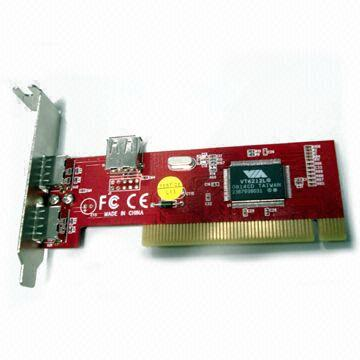
\includegraphics[height=70pt]{pictures/pci_card.jpg}}
                \fbox{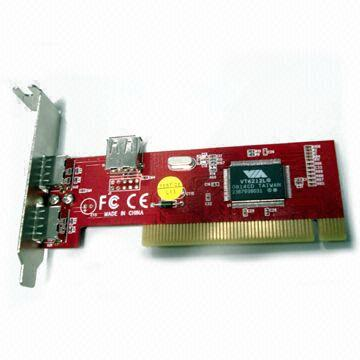
\includegraphics[scale=0.2]{pictures/pci_card.jpg}}
            \end{center}
            \scriptsize{
                Description du périphérique :
                \begin{itemize}
                    \item Registres ;
                    \item Algorithmes.
                \end{itemize}
            }
        }
    \end{column}

    % Center column for Middle-end (\rtx\ Maintainer)
    \begin{column}[c,T]{115pt}
        \uncover<2-> {
            \begin{center} \large{\itshape{Développeur \rtx}} \end{center}
            \scriptsize{
                Identification des sémantiques communes à tous les systèmes
                d'exploitation afin d'en tirer un modèle générique.
            }
        }
    \end{column}
    
    % Right column for Back-end (OS developer)
    \begin{column}[r,T]{115pt}
        \uncover<3-> {
            \begin{center} \large{\itshape{Développeur Système}} \end{center}
            \scriptsize{
                Code spécifique aux systèmes d'exploitation. Requiert des
                connaissances systèmes poussées.
            }
        }
    \end{column}

    \transdissolve<1>
    \transdissolve<2>
    \transdissolve<3>
\end{columns}
\end{frame}

\subsection{Le rôle de chaque partie du DSL}
\begin{frame}
\frametitle{Un DSL en trois parties}
\begin{columns}[c]
    
    \begin{column}[l,T]{115pt}
        \begin{center} \large{\itshape{Front-End}} \end{center}
        \scriptsize{
            \begin{center} Fichier \texttt{.rtx} \end{center}
            Il contient une description :
            \begin{itemize}
                \item Physique du matériel (registres) ;
                \item Algorithmique du pilote ;
                \item Une configuration (sous-systèmes à utiliser, informations
                                         spécifiques à chaque système
                                         d'exploitation...).
            \end{itemize}
        }
    \end{column}
    
    \begin{column}[c,T]{115pt}
        \begin{center} \large{\itshape{Middle-End}} \end{center}
        \scriptsize{
            \begin{center} Fichier \texttt{.rti} \end{center}
            Il contient des interfaces de sous-systèmes décrivant :
            \begin{itemize}
                \item Des Types ;
                \item Des Séquences ;
                \item Des variables de configuration.
            \end{itemize}
        }
    \end{column}
    
    \begin{column}[r,T]{115pt}
        \begin{center} \large{\itshape{Back-End}} \end{center}
        \scriptsize{
            \begin{center} Fichier \texttt{.blt} \end{center}
            Il permet d'implémenter le code système-spécifique correspondant
            aux interfaces associées. On y retrouvera :
            \begin{itemize}
                \item Des templates de type ;
                \item Des templates de séquence.
            \end{itemize}
            Chaque morceau de code C instrumenté qui s'y trouve est appelé
            ``placeHolder''.
        }
    \end{column}

\end{columns}
\transdissolve<1>
\end{frame}

\section{Problématiques de développement et solutions}

\subsection{Définition du langage de templates}
\begin{frame}
\frametitle{Comment faire un langage souple ?}
Il existe plusieurs besoins en plus de celui d'avoir un compilateur et un
langage évolutifs :
\begin{enumerate}[<+->]
    \item Implémenter facilement de nouvelles sémantiques ;
    \item Spécifier le système pour lequel on implémente le code ;
    \item Générer facilement du C à partir de ces implémentations ;
    \item Avoir un langage compréhensible.
\end{enumerate}
\end{frame}

\begin{frame}
\frametitle{Du langage souple aux templates}
\only<1-3> {
    Ceci impliquait donc un langage instrumentant le C contenant :
    \begin{enumerate}[<+->]
        \item Un moyen de sélectionner du code selon une configuration ;
        \item Une association un élément = une sémantique ;
        \item Un moyen de manipuler cette surcouche au C dans le C.
    \end{enumerate}
}
\only<4> {
    Se traduisant en un langage de templates contenant :
    \begin{enumerate}
        \item Un bloc ``with'' décrivant les conditions de sélection
            du code (configuration);
        \item Un bloc ``template'' implémentant une sémantique décrite dans
            une interface ;
        \item Une syntaxe ``placeHolder'' permettant de manipuler
            des données du C instrumenté dans le C.
    \end{enumerate}
}
\transdissolve<4>[duration=0.5]
\end{frame}

\subsection{Génération du code : technique de tissage d'ASTs}
\begin{frame}
\frametitle{Comment résoudre un template ?}
\only<1-6> {
    Un template ne peut pas :
    \begin{enumerate}[<+->]
        \item Être indépendant de son contexte ;
        \item Générer du code brut ;
        \item Générer quelque chose d'incompatible avec le C.
    \end{enumerate}
    \uncover<4-> {
        Il doit donc :
        \begin{enumerate}[<+->]
            \item Se résoudre à l'aide de paramètres facilement manipulables ;
            \item Générer quelque chose de compatible avec le C ;
            \item Utiliser une forme facilement manipulable.
        \end{enumerate}
    }
    \transdissolve<4>[duration=0.3]
}
\only<7> {
    Les solutions adoptées :
    \begin{enumerate}
        \item Mise en place d'un système de mapping de valeurs pour
            la résolution basé sur les paramètres du template ;
        \item Génération d'un AST C compatible.
    \end{enumerate}
}
\end{frame}

\subsection{Gestion de la bibliothèque de templates}
\begin{frame}
\frametitle{Accélérer le processus de génération}
\only<1-3> {
    Qu'est-ce qui rend le processus de génération lent ?
    \begin{enumerate}[<+->]
        \item Analyser/compiler un template a un coût ;
        \item Rechercher un template précis est donc lent ;
        \item Le but de rathaxes est d'être une bibliothèque de templates
            et de drivers prêts à être générés.
    \end{enumerate}
}
\only<4-6> {
    Quelques idées pour améliorer les choses :
    \begin{enumerate}
        \item<4-> La compilation d'un template génère un AST et un script
            CodeWorker ;
        \item<5-> Il faut maintenir un cache des templates compilés ;
        \item<6-> Ce cache doit se limiter à des fichiers à charger avec
            le moins d'opérations possibles.
    \end{enumerate}
}
\only<7-> {
    Le cache permet donc :
    \begin{enumerate}
        \item<7-> Accès rapide à un template en fonction de son prototype ;
        \item<8-> Chargement automatique du script et de l'arbre associés ;
        \item<9-> Au travers de la fonction template générée, une résolution
            facile du template utilisé.
    \end{enumerate}
}
\transdissolve<4>
\end{frame}


\subsection{Insertion de code spécifique : ajout de l'aspectuel}

\begin{frame}[containsverbatim]
\frametitle{Apparition de nouvelles problématiques}
\lstset{
    basicstyle=\color{black}\tiny\ttfamily,
    numberstyle=\tiny\ttfamily
}
Exemple de template tel que défini précédemment :
\begin{lstlisting}
with LKM
values OS=Linux, version>2.6.30
{
    template init(Context)
    {
        struct module mod =
        {
            .open = ????,
        };
        int templated_init()
        {
            // Do something here
        }
        module_init(templated_init);
    }
}
\end{lstlisting}
\end{frame}



\begin{frame}
\frametitle{Les manques des templates...}
Plusieurs problématiques apparaissent :
\begin{enumerate}
    \item Multiples insertions à un endroit précis par des sources
        différentes ;
    \item Rendre une insertion optionnelle ;
    \item Imaginer un modèle extensible résolvant ces problématiques.
\end{enumerate}
\end{frame}

\begin{frame}
\frametitle{...et donc la programmation aspectuelle}
\only<1> {
    % Les concepts
    Les intérêts de la Programmation Orientée Aspect :
    \begin{itemize}
        \item Séparer des éléments de métiers différents au sein d'un code ;
        \item Centré sur l'idée de tissage de code statique ou dynamique.
    \end{itemize}
}
\only<2> {
    % Le lexique
    Les mots clefs du paradigme :
    \begin{itemize}
        \item Aspect ;
        \item Greffon (ou advice) ;
        \item Point de coupe (ou pointcut) ;
        \item Point de jonction (ou joinpoint).
    \end{itemize}
}
\end{frame}


\begin{frame}
\frametitle{Arrivée de l'aspectuel dans le DSL}
Grâce à la Programmation Orientée Aspect, nous allons pouvoir :
\begin{enumerate}[<+->]
    \item Définir des points de coupe pour chaque élément nécéssitant de
        multiples insertions ;
    \item Ajouter un comportement par défaut pour chacun des points de coupe ;
    \item Permettre de définir des greffons (advices) dans les templates,
        pour spécialiser selon les situations:
        \begin{enumerate}
            \item Définition de fonction ;
            \item Définition de variables globales ;
            \item Appel de fonction ;
            \item Attribution de pointeur sur fonction ;
            \item etc...
        \end{enumerate}
\end{enumerate}
\end{frame}

\begin{frame}
\frametitle{Implémentation dans le langage}
\begin{enumerate}[<+->]
    \item Ajout de \emph{placeHolders} point de coupe : les ``pointcuts'' ;
    \item Ajout d'un bloc ``default'' dans le point de coupe ;
    \item Changements du template :
        \begin{enumerate}
            \item Déplacement du code dans des greffons : les ``chunks'' ;
            \item Ajout de greffons spécifiques pour cas particuliers
                (builtins).
        \end{enumerate}
\end{enumerate}
\end{frame}

\begin{frame}
\frametitle{Implémentation dans le cache}
\begin{enumerate}[<+->]
    \item Recherche par template (ex: appel d'un template en \rtx) ;
    \item Recherche par greffon (résolution d'un pointcut) ;
    \item Adaptabilité de la génération :
        génération de script et AST par configuration.
\end{enumerate}
\end{frame}

\begin{frame}
\frametitle{Pour résumer...}
\begin{itemize}
    \item Description des ``aspects'' du compilateur par des interfaces ;
    \item Implémentation des templates respectant ces interfaces ;
    \item Le langage utilisateur n'est qu'une suite de tissage de ces aspects.
\end{itemize}
\end{frame}

\section{Présentation du langage}

\begin{frame}
\frametitle{Syntaxe d'une interface de sous-système}
\only<1> {
    Fournit cinq types d'éléments :
    \begin{itemize}
        \item Types ;
        \item Séquences ;
        \item Variables ;
        \item Pointcuts ;
        \item Chunks.
    \end{itemize}
}
\only<2> {
    Quatre mots clefs pour identifier qui implémente quoi.
    Ces mot clefs s'appliquent aux séquences, types et variables.
    \begin{itemize}
        \item provided ;
        \item required ;
        \item optional ;
        \item auto.
    \end{itemize}
}
\only<3> {
    Deux mots clefs pour identifier qui implémente quoi pour la partie
    aspectuelle de \rtx.
    \begin{itemize}
        \item provided ;
        \item use.
    \end{itemize}
}
\only<4> {
    Tableau de croisement des mot clefs avec leur implication pour le
    Front-End et le Back-End :
    \center {
    \begin{tabular}{|l|c|c|c|}
        \hline
             & Front  & Back & Generation  \\
        \hline
        \textcolor{tblB}{auto}     & \textcolor{tblR}{Non}
            & \textcolor{tblG}{Oui} & \textcolor{tblG}{Oui} \\
        \hline
        \textcolor{tblB}{provided} & \textcolor{tblR}{Non}
            & \textcolor{tblG}{Oui} & Si utilisé  \\
        \hline
        \textcolor{tblB}{required} & \textcolor{tblG}{Oui}
            & \textcolor{tblG}{Oui} & \textcolor{tblG}{Oui} \\
        \hline
        \textcolor{tblB}{optional} & Possible
            & Oui si redéfini & Si utilisé  \\
        \hline
    \end{tabular}
    }
}
\transdissolve<2>[duration=0.4]
\transdissolve<3>[duration=0.2]

%\transwipe<2>[direction=90]
\end{frame}


\begin{frame}[containsverbatim]
\frametitle{Exemple d'interface (\texttt{.rti})}
\lstset{
    basicstyle=\color{black}\tiny\ttfamily,
    numberstyle=\tiny\ttfamily
}
\begin{lstlisting}
/*
 * This interface describes the basic needs for
 * any loadable kernel module
 */
   interface LKM : Builtins
   {
       builtin  type       Device;

       provided pointcut   include_dependencies;
       provided pointcut   global_data_declaration;
       provided pointcut   code_declaration;
       provided pointcut   lkm_base_code_definition;

       provided sequence   load()
       {
           provided pointcut   lkm_init_fptrs;
           use      pointcut   lkm_base_code_definition;
       }

       provided sequence   unload()
       {
           provided pointcut   unload_setup;
           use      pointcut   lkm_base_code_definition;
       }
       required variable Builtins::string OS;
       required variable Builtins::serial version;
   }
\end{lstlisting}
\end{frame}

\begin{frame}[containsverbatim]
\frametitle{Exemple de template (\texttt{.blt})}
\lstset{
    basicstyle=\color{black}\tiny\ttfamily,
    numberstyle=\tiny\ttfamily
}
\begin{lstlisting}
with LKM
{
    ${pointcut include_dependencies};
    ${pointcut global_data_declaration};
    ${pointcut code_declaration};
    ${pointcut lkm_base_code_definition};
}
with LKM
values OS=Linux, version>=2.6.24
{
    template sequence load()
    {
        chunk lkm_base_code_definition
        {
            int modentry()
            { /* Init some stuff here */ }
            module_init(modentry);
        }
        chunk global_data_declaration
        {
            struct module myModule = {
                ${pointcut lkm_init_fptrs
                  default:
                      .module_open = NULL;
                },
            };
        }
    }
}
\end{lstlisting}
\end{frame}

\begin{frame}[containsverbatim]
\frametitle{Exemple d'implémentation de pilote (\texttt{.rtx})}
\lstset{
    basicstyle=\color{black}\tiny\ttfamily,
    numberstyle=\tiny\ttfamily
}
\begin{lstlisting}
device myDriver
{
    // Here the driver's registers description
}

driver myDriver
{
    Userland::open(Context ctx) {
        log("Opening device...\n");
    }
    Userland::close(Context ctx) {
        log("Closing device...\n");
    }
}

configuration
{
    LKM::devices = myDriver;
    LKM::arch = x86;
    LKM::OS=Linux {
        LKM::version = 2.6.34;
    }
    LKM::OS=Windows7 {
    }
};
\end{lstlisting}
\end{frame}




\section{Un compilateur hors normes}

\subsection{Le langage \rtx}
\begin{frame}
\frametitle{La différence avec un langage structuré}
\begin{itemize}[<+->]
    \item Le code écrit n'a aucun rapport avec le code généré en termes
        de flux d'exécution ;
    \item Correspondance complexe entre declaration rathaxes et expression C.
\end{itemize}
\end{frame}

\begin{frame}
\frametitle{Du langage au compilateur}
\uncover<1-> {
    Trois parties dans le DSL :
    \begin{itemize}
        \item Indépendantes pour la compilation ;
        \item Liées pour la génération.
    \end{itemize}
}
\uncover<2> {
    Le DSL est aussi un sur-ensemble du C :
    \begin{itemize}
        \item Gestion du langage C ;
        \item Instrumentalisation du C ;
        \item Interfacage pour la génération entre
            l'AST \rtx\ et l'AST du C.
    \end{itemize}
}
\end{frame}


\subsection{Un compilo pour les traduire tous}
\begin{frame}
\frametitle{Les composants}
\begin{itemize}[<+->]
    \item CNorm ;
    \item rtxParse : syntaxe du DSL ;
    \item RtxNode : normalisation des nodes de l'AST ;
    \item rtxLink : cache des interfaces et templates enregistrés ;
    \item rtxTpl : résolution des templates ;
    \item Tool : génération de fichiers annexes (\texttt{.inf},
                 \texttt{Makefiles}, etc...).
\end{itemize}
\end{frame}


\begin{frame}
\frametitle{Compilation du Middle-End}
\begin{itemize}[<+->]
    \item Analyse du code ;
    \item Validation des dépendances ;
    \item Validation de l'interface elle-même ;
    \item Enregistrement dans le cache.
\end{itemize}
\end{frame}

\begin{frame}
\frametitle{Compilation du Back-End}
\begin{itemize}[<+->]
    \item Analyse du code C instrumenté ;
    \item Validation des prototypes de templates ;
    \item Validation de la présence des éléments de programmation aspectuelle
            requis par l'interface ;
    \item Extraction des PlaceHolders ;
    \item Enregistrement dans le cache.
\end{itemize}
\end{frame}

\subsection{Et dans les ténèbres les lier.}
\begin{frame}
\frametitle{Compilation du Front-End}
\begin{itemize}[<+->]
    \item Analyse du code ;
    \item Vérification des types utilisés à l'aide des interfaces ;
    \item Sélection des templates utilisés (appels, redéfinitions, etc...) depuis le cache ;
    \item Première étape de génération : LKM ;
    \item Résolution des \emph{placeHolders} (templates/chunks/pointcuts) ;
    \item Assemblage et génération.
\end{itemize}
\end{frame}

\section{Conclusion}
\begin{frame}
\frametitle{Merci}
Questions ?
\end{frame}

\end{document}
